\documentclass{article}

\usepackage{graphicx}
\usepackage{tikz}
\usepackage{tikzsymbols}
\usetikzlibrary{calc,patterns,shapes.geometric}
\pagestyle{empty}
\usepackage[margin=0pt]{geometry}
\geometry{papersize={14in,12in}}

\def\centerarc[#1](#2)(#3:#4:#5){\draw[#1] ($(#2)+({#5*cos(#3)},{#5*sin(#3)})$) arc (#3:#4:#5);}

\begin{document}
	\begin{figure}
		\centering
		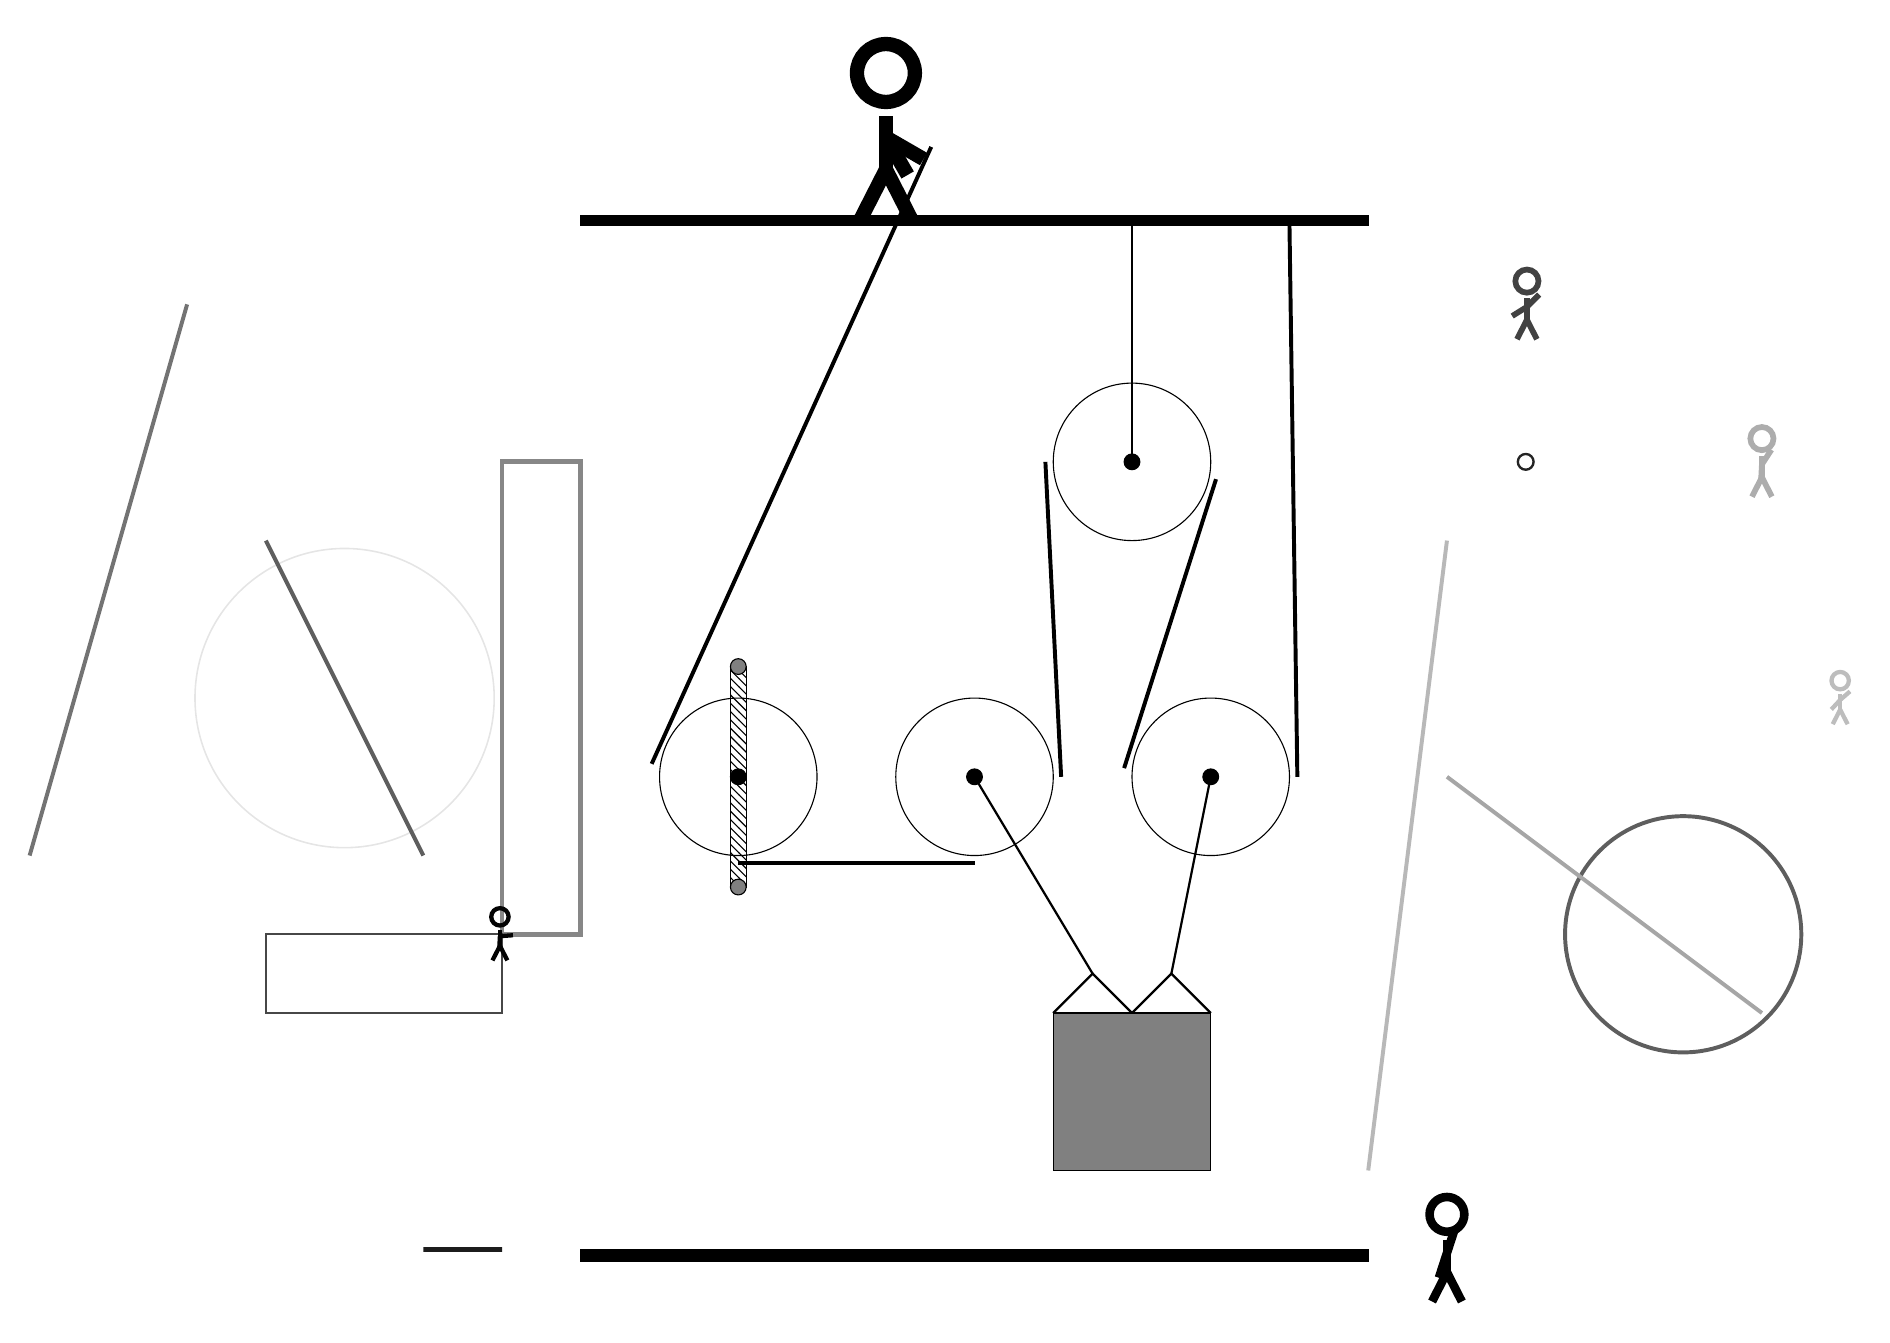
\begin{tikzpicture}
			%%%%% START %%%%%
			
			\draw[fill=black] (-4, 10) rectangle (6, 10.125);
			
			\draw (1, 3.0) circle (1);
			\draw[fill=black] (1, 3.0) circle (0.1);
			
			\draw (3, 7.0) circle (1);
			\draw[fill=black] (3, 7.0) circle (0.1);
			\draw[thick] (3, 7.0) -- (3, 10);
			
			\draw (4, 3.0) circle (1);
			\draw[fill=black] (4, 3.0) circle (0.1);
			
			\draw[thick] (4, 3.0) -- (3.5, 0.5);
			\draw[thick] (1, 3.0) -- (2.5, 0.5);
			\draw[thick]  (2, 0) -- (2.5, 0.5) -- (3, 0);
			\draw[thick]  (3, 0) -- (3.5, 0.5) -- (4, 0);
			\draw[fill=black!50] (2, 0) rectangle (4, -2);
			
			\draw (-2, 3.0) circle (1);
			\draw[fill=black] (-2, 3.0) circle (0.1);
			\draw[pattern=north west lines, pattern color=black] (-2.1, 4.4) rectangle (-1.9, 1.6);
			\draw[fill=black!50] (-2, 4.4) circle (0.1);
			\draw[fill=black!50] (-2, 1.6) circle (0.1);
			
			\draw[line width=0.5mm] (0.45, 11) -- (-3.1, 3.165);
			\centerarc[line width=0.5mm](-2, 3.0)(160:270:1.1);
			\draw[line width=0.5mm](-2, 1.9) -- (1, 1.9);
			\centerarc[line width=0.5mm](1, 3.0)(270:360:1.1);
			\draw[line width=0.5mm] (2.1, 3.0) -- (1.9, 7.0);
			\centerarc[line width=0.5mm](3, 7.0)(-20:180:1.1);
			\draw[line width=0.5mm](4.067, 6.78) -- (2.9, 3.11);
			\centerarc[line width=0.5mm](4, 3.0)(160:360:1.1);
			\draw[line width=0.5mm](5.1, 3.0) -- (5.0, 10);
			
			\node at (-0.07, 11.2) {\Strichmaxerl[10][120][-30]};
			
			\draw [line width=0.2mm, color=black!10](-7, 4) circle (1.9);
			
			\node[line width=0.4mm, color=black!26] at (12, 4) {\Strichmaxerl[3][47][41]};
			\draw[line width=0.6mm, color=black!47] (-4, 1) rectangle (-5, 7);
			\draw [line width=0.5mm, color=black!63](10, 1) circle (1.5);
			
			\node[line width=0.6mm, color=black!74] at (8, 9) {\Strichmaxerl[4][32][45]};
			\draw[line width=0.5mm, color=black!55](-9, 9) -- (-11, 2);
			
			\draw[line width=0.7mm, color=black!89] (-5, -3) rectangle (-6, -3);
			\node[line width=0.5mm, color=black!100] at (7, -3) {\Strichmaxerl[6][72][72]};
			\draw[line width=0.3mm, color=black!72] (-5, 1) rectangle (-8, 0);
			\draw[line width=0.5mm, color=black!28](6, -2) -- (7, 6);
			\node[line width=0.5mm, color=black!32] at (11, 7) {\Strichmaxerl[4][87][57]};
			\node[line width=0.5mm, color=black!99] at (-5, 1) {\Strichmaxerl[3][87][4]};
			\draw[line width=0.5mm, color=black!63](-6, 2) -- (-8, 6);
			\draw[line width=0.5mm, color=black!35](7, 3) -- (11, 0);
			\draw [line width=0.3mm, color=black!86](8, 7) circle (0.1);
			
			\draw[fill=black] (-4, -3) rectangle (6, -3.15);
			
			%%%%% END %%%%%
		\end{tikzpicture}
	\end{figure}	
\end{document}